%Documentação do Trabalho Prático 0 de AEDSIII
%Édipo Fernandes Vieira de Oliveira - 2011054324
\documentclass[12pt, a4paper]{article}
\usepackage[utf8]{inputenc}
\usepackage[brazil]{babel} %idioma
\usepackage{ae} %caracteres especiais
\usepackage{amsmath, amsfonts, amssymb}
\usepackage{enumerate}
\usepackage[tmargin=2cm, bmargin=2cm, lmargin=2cm, rmargin=2cm]{geometry}
\usepackage{graphicx}
\usepackage[lined,algonl,ruled]{algorithm2e} %Para acrescentar algorithm
\begin{document}

 %capa

 \title{Trabalho Prático 1 \\ Rede Social de Pesquisadores \\}
 \author{Édipo Fernandes Vieira de Oliveira - 2011054324\\ Diego Henrique de Castro Aniceto - 2011054286\\Departamento de Ciência da Computação -- Universidade Federal de Minas Gerais\\}
  \maketitle

 %\newpage
 %sumario
  %use o section

\textbf{\textit \\Resumo: }
\textit{\\ Este relatório descreve a implementação da solução proposta para o o problema de manipulação de e armazenamento de dados de uma rede social de pesquisadores. Para que fosse possivel essa implemetação foi utilizado a linguagem Java de programação além de teorias de Orientação a Objeto e Modularização.\\
  O resultado obtido foi satisfatório, tanto em relação a solução do problema, quanto aos conceitos envolvidos.}
\section*{1. Introdução}

  Este trabalho tem como objetivo, introduzir os principais conceitos da Programação Orientada ao Objeto e modularização de código. Para que estes fossem exercitados foi proposto a solução de um problemas de manipulação e armazenamento de dados referentes a uma rede social de pesquisadores onde eles podem se relacionar através de artigos publicados, podem publicar seus artigos desenvidos, entre outras coisas \\\\
  A modelagem do problema gira em torno de três entidades principais, que são os Pesquisadores, os Veiculos de Comunicação e os Artigos, e a partir delas e dos arquivos de entradas disponibilizados, e a partir disso realizar os calculos solictidos pela especificação do trabalho, que são: o calculo de popularidade de cada Pesquisador, o fator de impacto de cada Veiculo de Comunicação, e a pontuação de cada Artigo.

  \begin{itemize}
  \item A seção 2 discute detalhes de implementação.
  \item A seção 3 traz os testes realizados para verificar a solução do trabalho, bem como a saída gerada
  \item A seção 4 apresenta uma breve conclusão sobre o trabalho.
  \item E por fim a seção 5 traz as referências bibliográficas.
\end{itemize}

%% Implementação %%
\section*{2. Implementação}
  \subsection*{2.1. Modularização e Encapsulamento}
  Como dito na secção anterior, a implementação da solução gira em torno das entidades Pesquisador, Veiculos de Cominicação e Artigo, estas foram mapeadas através da implementação de classes Java, onde seus atributos e metódos identificam-nas. Porém, apenas elas não são o suficiente para a resolução do problema, outras classes dependentes delas são necessarias para que a solução obtivesse êxito. \\\\
  Das classes-entidades citadas acima, uma merece atenção especial, a entidade Artigo, pois ela se relaciona diretamente com as classes \textit{Veiculos de Cominicação} e \textit{Pesquisador}, além disso é preciso identificar as citações feitas nos artigos em questão. Afim de modularizar o código e facilitar seu entendimento as classes fora estruturadas da seguinte forma:

  \begin{figure}[!htb]
   \centering
    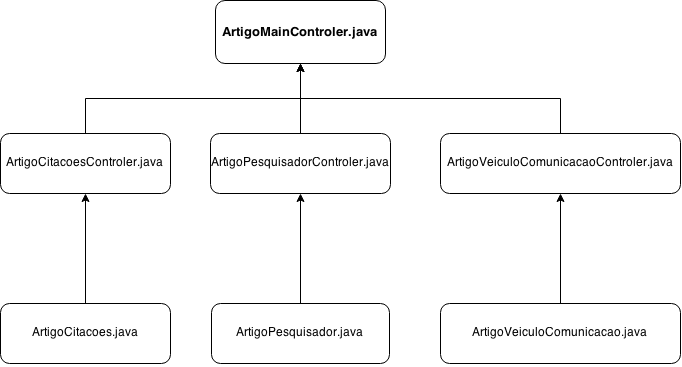
\includegraphics[scale=0.5]{Artigo}
    \caption{Estrutura de Dependência de Artigo}
   \label{Rotulo}
  \end{figure}
  Como pode ser visto no diagrama acima, a classe \textbf{ArtigoMainControle.java} faz o encapsulamento das demais classes, fornecendo o conjunto de todas as operações necessárias envolvendo um Artigo, não sendo necessario assim nenhuma altaração nas classes bases.\\\\
  A modularização das entidades Pesquisador e Veiculo de Comunicação foram feitas de forma similar a classe Artigo, porém de forma mais simples pois essas classes não tem dependências de demais classes, o que facilita o reuso e a manutenção destas.

  \subsection*{2.2. Conceitos OO}
    Para a modularização e o encapsulamento das classes fossem possíveis, foi necessária a implementação dos conceitos de \textit{Orientação a Objeto}.\\\\
    O conceito utilizado para realizar o relacionamento entre as classes foi o de \textbf{Composição} onde temos uma classe que funciona como o \textit{todo} e classes que funcionam como uma parte deste todo, por exemplo, a classe \textbf{PesquisadorControle} (responsável pela implementação dos metódos referentes a entidade Pesquisador) é o todo e a classe \textbf{Pesquisador} é parte da classe \textbf{PesquisadorControle}.
    Foi utilizado também o conceito de Objeto, que foi utilizado para que o acesso as classes dependentes fosse possível.

  \subsection*{2.3. Calculos e Execução}
    O principal objetivo do trabalho era fornecer uma lista com a popularidade de cada pesquisador, o fator de impacto de cada veiculo de comunicação e a pontuação de cada artigo. Para resolver esses problemas, foi criada uma classe especifica que processa todos esses dados e gera os dados solicitados.\\\\
    Esta classe é composta por objetos de todas as classes \textbf{Controle} que fornecem as operações de suas respectivas entidades, tornando possível o processamento dos dados e o fornecimento das respostas.\\\\
    Para que a solução fosse executada, foi desenvolvida uma classe principal, \textbf{MainClass}, que contem um construtor e um objeto da classe \textbf{Resultado} que realiza os cálculos necessários pra solucionar o problema proposto.


%% Testes %%
\section*{3. Testes}

%% Conclusão %%
\section*{4. Conclusão}


%% Referencias %%
\section*{5. Referências bibliográficas}
\end{document}
